\pdfoutput=1
%% Author: PGL  Porta Mana
%% Created: 2015-05-01T20:53:34+0200
%% Last-Updated: 2020-01-16T21:32:23+0100
%%%%%%%%%%%%%%%%%%%%%%%%%%%%%%%%%%%%%%%%%%%%%%%%%%%%%%%%%%%%%%%%%%%%%%%%%%%%
\newif\ifarxiv
\arxivfalse
\ifarxiv\pdfmapfile{+classico.map}\fi
\newif\ifafour
\afourfalse% true = A4, false = A5
\newif\iftypodisclaim % typographical disclaim on the side
\typodisclaimtrue
\newcommand*{\memfontfamily}{zplx}
\newcommand*{\memfontpack}{newpxtext}
\documentclass[\ifafour a4paper,12pt,\else a5paper,10pt,\fi%extrafontsizes,%
onecolumn,oneside,article,%french,italian,german,swedish,latin,
british%
]{memoir}
\newcommand*{\firstdraft}{17 October 2019}
\newcommand*{\firstpublished}{17 October 2019}
\newcommand*{\updated}{\ifarxiv***\else\today\fi}
\newcommand*{\propertitle}{Notes on inferring connectivity\\ (Bente's problem) [draft]%\\{\large ***}%
}% title uses LARGE; set Large for smaller
\newcommand*{\pdftitle}{\propertitle}
\newcommand*{\headtitle}{Connectivity and Bente's problem}
\newcommand*{\pdfauthor}{P.G.L.  Porta Mana, B. Jacobsen}
\newcommand*{\headauthor}{Porta Mana, Jacobsen}
\newcommand*{\reporthead}{\ifarxiv\else Open Science Framework \href{https://doi.org/10.31219/osf.io/***}{\textsc{doi}:10.31219/osf.io/***}\fi}% Report number

%%%%%%%%%%%%%%%%%%%%%%%%%%%%%%%%%%%%%%%%%%%%%%%%%%%%%%%%%%%%%%%%%%%%%%%%%%%%
%%% Calls to packages (uncomment as needed)
%%%%%%%%%%%%%%%%%%%%%%%%%%%%%%%%%%%%%%%%%%%%%%%%%%%%%%%%%%%%%%%%%%%%%%%%%%%%

%\usepackage{pifont}

%\usepackage{fontawesome}

\usepackage[T1]{fontenc} 
\input{glyphtounicode} \pdfgentounicode=1

\usepackage[utf8]{inputenx}

%\usepackage{newunicodechar}
% \newunicodechar{Ĕ}{\u{E}}
% \newunicodechar{ĕ}{\u{e}}
% \newunicodechar{Ĭ}{\u{I}}
% \newunicodechar{ĭ}{\u{\i}}
% \newunicodechar{Ŏ}{\u{O}}
% \newunicodechar{ŏ}{\u{o}}
% \newunicodechar{Ŭ}{\u{U}}
% \newunicodechar{ŭ}{\u{u}}
% \newunicodechar{Ā}{\=A}
% \newunicodechar{ā}{\=a}
% \newunicodechar{Ē}{\=E}
% \newunicodechar{ē}{\=e}
% \newunicodechar{Ī}{\=I}
% \newunicodechar{ī}{\={\i}}
% \newunicodechar{Ō}{\=O}
% \newunicodechar{ō}{\=o}
% \newunicodechar{Ū}{\=U}
% \newunicodechar{ū}{\=u}
% \newunicodechar{Ȳ}{\=Y}
% \newunicodechar{ȳ}{\=y}

\newcommand*{\bmmax}{0} % reduce number of bold fonts, before font packages
\newcommand*{\hmmax}{0} % reduce number of heavy fonts, before font packages

\usepackage{textcomp}

%\usepackage[normalem]{ulem}% package for underlining
% \makeatletter
% \def\ssout{\bgroup \ULdepth=-.35ex%\UL@setULdepth
%  \markoverwith{\lower\ULdepth\hbox
%    {\kern-.03em\vbox{\hrule width.2em\kern1.2\p@\hrule}\kern-.03em}}%
%  \ULon}
% \makeatother

\usepackage{amsmath}

\usepackage{mathtools}
\addtolength{\jot}{\jot} % increase spacing in multiline formulae
\setlength{\multlinegap}{0pt}

%\usepackage{empheq}% automatically calls amsmath and mathtools
%\newcommand*{\widefbox}[1]{\fbox{\hspace{1em}#1\hspace{1em}}}

%%%% empheq above seems more versatile than these:
%\usepackage{fancybox}
%\usepackage{framed}

% \usepackage[misc]{ifsym} % for dice
% \newcommand*{\diceone}{{\scriptsize\Cube{1}}}

\usepackage{amssymb}

\usepackage{amsxtra}

\usepackage[main=british,french,italian,german,swedish,latin,esperanto]{babel}\selectlanguage{british}
\newcommand*{\langfrench}{\foreignlanguage{french}}
\newcommand*{\langgerman}{\foreignlanguage{german}}
\newcommand*{\langitalian}{\foreignlanguage{italian}}
\newcommand*{\langswedish}{\foreignlanguage{swedish}}
\newcommand*{\langlatin}{\foreignlanguage{latin}}
\newcommand*{\langnohyph}{\foreignlanguage{nohyphenation}}

\usepackage[autostyle=false,autopunct=false,english=british]{csquotes}
\setquotestyle{british}

\usepackage{amsthm}
\newcommand*{\QED}{\textsc{q.e.d.}}
\renewcommand*{\qedsymbol}{\QED}
\theoremstyle{remark}
\newtheorem{note}{Note}
\newtheorem*{remark}{Note}
\newtheoremstyle{innote}{\parsep}{\parsep}{\footnotesize}{}{}{}{0pt}{}
\theoremstyle{innote}
\newtheorem*{innote}{}

\usepackage[shortlabels,inline]{enumitem}
\SetEnumitemKey{para}{itemindent=\parindent,leftmargin=0pt,listparindent=\parindent,parsep=0pt,itemsep=\topsep}
% \begin{asparaenum} = \begin{enumerate}[para]
%     \begin{inparaenum} = \begin{enumerate*}
\setlist{itemsep=0pt,topsep=\parsep}
\setlist[enumerate,2]{label=\alph*.}
\setlist[enumerate]{label=\arabic*.,leftmargin=1.5\parindent}
\setlist[itemize]{leftmargin=1.5\parindent}
\setlist[description]{leftmargin=1.5\parindent}
% old alternative:
% \setlist[enumerate,2]{label=\alph*.}
% \setlist[enumerate]{leftmargin=\parindent}
% \setlist[itemize]{leftmargin=\parindent}
% \setlist[description]{leftmargin=\parindent}

\usepackage[babel,theoremfont,largesc]{newpxtext}

\usepackage[bigdelims,nosymbolsc%,smallerops % probably arXiv doesn't have it
]{newpxmath}
\linespread{1.083}%\useosf
%% smaller operators for old version of newpxmath
\makeatletter
\def\re@DeclareMathSymbol#1#2#3#4{%
    \let#1=\undefined
    \DeclareMathSymbol{#1}{#2}{#3}{#4}}
%\re@DeclareMathSymbol{\bigsqcupop}{\mathop}{largesymbols}{"46}
%\re@DeclareMathSymbol{\bigodotop}{\mathop}{largesymbols}{"4A}
\re@DeclareMathSymbol{\bigoplusop}{\mathop}{largesymbols}{"4C}
\re@DeclareMathSymbol{\bigotimesop}{\mathop}{largesymbols}{"4E}
\re@DeclareMathSymbol{\sumop}{\mathop}{largesymbols}{"50}
\re@DeclareMathSymbol{\prodop}{\mathop}{largesymbols}{"51}
\re@DeclareMathSymbol{\bigcupop}{\mathop}{largesymbols}{"53}
\re@DeclareMathSymbol{\bigcapop}{\mathop}{largesymbols}{"54}
%\re@DeclareMathSymbol{\biguplusop}{\mathop}{largesymbols}{"55}
\re@DeclareMathSymbol{\bigwedgeop}{\mathop}{largesymbols}{"56}
\re@DeclareMathSymbol{\bigveeop}{\mathop}{largesymbols}{"57}
%\re@DeclareMathSymbol{\bigcupdotop}{\mathop}{largesymbols}{"DF}
%\re@DeclareMathSymbol{\bigcapplusop}{\mathop}{largesymbolsPXA}{"00}
%\re@DeclareMathSymbol{\bigsqcupplusop}{\mathop}{largesymbolsPXA}{"02}
%\re@DeclareMathSymbol{\bigsqcapplusop}{\mathop}{largesymbolsPXA}{"04}
%\re@DeclareMathSymbol{\bigsqcapop}{\mathop}{largesymbolsPXA}{"06}
\re@DeclareMathSymbol{\bigtimesop}{\mathop}{largesymbolsPXA}{"10}
%\re@DeclareMathSymbol{\coprodop}{\mathop}{largesymbols}{"60}
%\re@DeclareMathSymbol{\varprod}{\mathop}{largesymbolsPXA}{16}
\makeatother
%%
%% With euler font cursive for Greek letters - the [1] means 100% scaling
\DeclareFontFamily{U}{egreek}{\skewchar\font'177}%
\DeclareFontShape{U}{egreek}{m}{n}{<-6>s*[1]eurm5 <6-8>s*[1]eurm7 <8->s*[1]eurm10}{}%
\DeclareFontShape{U}{egreek}{m}{it}{<->s*[1]eurmo10}{}%
\DeclareFontShape{U}{egreek}{b}{n}{<-6>s*[1]eurb5 <6-8>s*[1]eurb7 <8->s*[1]eurb10}{}%
\DeclareFontShape{U}{egreek}{b}{it}{<->s*[1]eurbo10}{}%
\DeclareSymbolFont{egreeki}{U}{egreek}{m}{it}%
\SetSymbolFont{egreeki}{bold}{U}{egreek}{b}{it}% from the amsfonts package
\DeclareSymbolFont{egreekr}{U}{egreek}{m}{n}%
\SetSymbolFont{egreekr}{bold}{U}{egreek}{b}{n}% from the amsfonts package
% Take also \sum, \prod, \coprod symbols from Euler fonts
\DeclareFontFamily{U}{egreekx}{\skewchar\font'177}
\DeclareFontShape{U}{egreekx}{m}{n}{%
       <-7.5>s*[0.9]euex7%
    <7.5-8.5>s*[0.9]euex8%
    <8.5-9.5>s*[0.9]euex9%
    <9.5->s*[0.9]euex10%
}{}
\DeclareSymbolFont{egreekx}{U}{egreekx}{m}{n}
\DeclareMathSymbol{\sumop}{\mathop}{egreekx}{"50}
\DeclareMathSymbol{\prodop}{\mathop}{egreekx}{"51}
\DeclareMathSymbol{\coprodop}{\mathop}{egreekx}{"60}
\makeatletter
\def\sum{\DOTSI\sumop\slimits@}
\def\prod{\DOTSI\prodop\slimits@}
\def\coprod{\DOTSI\coprodop\slimits@}
\makeatother
% Greek letters not usually given in LaTeX.
\DeclareMathSymbol{\varpartial}{\mathalpha}{egreeki}{"40}
\DeclareMathSymbol{\partialup}{\mathalpha}{egreekr}{"40}
\DeclareMathSymbol{\alpha}{\mathalpha}{egreeki}{"0B}
\DeclareMathSymbol{\beta}{\mathalpha}{egreeki}{"0C}
\DeclareMathSymbol{\gamma}{\mathalpha}{egreeki}{"0D}
\DeclareMathSymbol{\delta}{\mathalpha}{egreeki}{"0E}
\DeclareMathSymbol{\epsilon}{\mathalpha}{egreeki}{"0F}
\DeclareMathSymbol{\zeta}{\mathalpha}{egreeki}{"10}
\DeclareMathSymbol{\eta}{\mathalpha}{egreeki}{"11}
\DeclareMathSymbol{\theta}{\mathalpha}{egreeki}{"12}
\DeclareMathSymbol{\iota}{\mathalpha}{egreeki}{"13}
\DeclareMathSymbol{\kappa}{\mathalpha}{egreeki}{"14}
\DeclareMathSymbol{\lambda}{\mathalpha}{egreeki}{"15}
\DeclareMathSymbol{\mu}{\mathalpha}{egreeki}{"16}
\DeclareMathSymbol{\nu}{\mathalpha}{egreeki}{"17}
\DeclareMathSymbol{\xi}{\mathalpha}{egreeki}{"18}
\DeclareMathSymbol{\omicron}{\mathalpha}{egreeki}{"6F}
\DeclareMathSymbol{\pi}{\mathalpha}{egreeki}{"19}
\DeclareMathSymbol{\rho}{\mathalpha}{egreeki}{"1A}
\DeclareMathSymbol{\sigma}{\mathalpha}{egreeki}{"1B}
 \DeclareMathSymbol{\tau}{\mathalpha}{egreeki}{"1C}
\DeclareMathSymbol{\upsilon}{\mathalpha}{egreeki}{"1D}
\DeclareMathSymbol{\phi}{\mathalpha}{egreeki}{"1E}
\DeclareMathSymbol{\chi}{\mathalpha}{egreeki}{"1F}
\DeclareMathSymbol{\psi}{\mathalpha}{egreeki}{"20}
\DeclareMathSymbol{\omega}{\mathalpha}{egreeki}{"21}
\DeclareMathSymbol{\varepsilon}{\mathalpha}{egreeki}{"22}
\DeclareMathSymbol{\vartheta}{\mathalpha}{egreeki}{"23}
\DeclareMathSymbol{\varpi}{\mathalpha}{egreeki}{"24}
\let\varrho\rho 
\let\varsigma\sigma
 \let\varkappa\kappa
\DeclareMathSymbol{\varphi}{\mathalpha}{egreeki}{"27}
%
\DeclareMathSymbol{\varAlpha}{\mathalpha}{egreeki}{"41}
\DeclareMathSymbol{\varBeta}{\mathalpha}{egreeki}{"42}
\DeclareMathSymbol{\varGamma}{\mathalpha}{egreeki}{"00}
\DeclareMathSymbol{\varDelta}{\mathalpha}{egreeki}{"01}
\DeclareMathSymbol{\varEpsilon}{\mathalpha}{egreeki}{"45}
\DeclareMathSymbol{\varZeta}{\mathalpha}{egreeki}{"5A}
\DeclareMathSymbol{\varEta}{\mathalpha}{egreeki}{"48}
\DeclareMathSymbol{\varTheta}{\mathalpha}{egreeki}{"02}
 \DeclareMathSymbol{\varIota}{\mathalpha}{egreeki}{"49}
\DeclareMathSymbol{\varKappa}{\mathalpha}{egreeki}{"4B}
\DeclareMathSymbol{\varLambda}{\mathalpha}{egreeki}{"03}
\DeclareMathSymbol{\varMu}{\mathalpha}{egreeki}{"4D}
\DeclareMathSymbol{\varNu}{\mathalpha}{egreeki}{"4E}
\DeclareMathSymbol{\varXi}{\mathalpha}{egreeki}{"04}
\DeclareMathSymbol{\varOmicron}{\mathalpha}{egreeki}{"4F}
\DeclareMathSymbol{\varPi}{\mathalpha}{egreeki}{"05}
\DeclareMathSymbol{\varRho}{\mathalpha}{egreeki}{"50}
\DeclareMathSymbol{\varSigma}{\mathalpha}{egreeki}{"06}
\DeclareMathSymbol{\varTau}{\mathalpha}{egreeki}{"54}
\DeclareMathSymbol{\varUpsilon}{\mathalpha}{egreeki}{"07}
\DeclareMathSymbol{\varPhi}{\mathalpha}{egreeki}{"08}
\DeclareMathSymbol{\varChi}{\mathalpha}{egreeki}{"58}
\DeclareMathSymbol{\varPsi}{\mathalpha}{egreeki}{"09}
\DeclareMathSymbol{\varOmega}{\mathalpha}{egreeki}{"0A} 
%
\DeclareMathSymbol{\Alpha}{\mathalpha}{egreekr}{"41}
\DeclareMathSymbol{\Beta}{\mathalpha}{egreekr}{"42}
\DeclareMathSymbol{\Gamma}{\mathalpha}{egreekr}{"00}
\DeclareMathSymbol{\Delta}{\mathalpha}{egreekr}{"01}
\DeclareMathSymbol{\Epsilon}{\mathalpha}{egreekr}{"45}
\DeclareMathSymbol{\Zeta}{\mathalpha}{egreekr}{"5A}
\DeclareMathSymbol{\Eta}{\mathalpha}{egreekr}{"48}
\DeclareMathSymbol{\Theta}{\mathalpha}{egreekr}{"02}
\DeclareMathSymbol{\Iota}{\mathalpha}{egreekr}{"49}
\DeclareMathSymbol{\Kappa}{\mathalpha}{egreekr}{"4B}
\DeclareMathSymbol{\Lambda}{\mathalpha}{egreekr}{"03}
\DeclareMathSymbol{\Mu}{\mathalpha}{egreekr}{"4D}
\DeclareMathSymbol{\Nu}{\mathalpha}{egreekr}{"4E}
\DeclareMathSymbol{\Xi}{\mathalpha}{egreekr}{"04}
\DeclareMathSymbol{\Omicron}{\mathalpha}{egreekr}{"4F}
\DeclareMathSymbol{\Pi}{\mathalpha}{egreekr}{"05}
\DeclareMathSymbol{\Rho}{\mathalpha}{egreekr}{"50}
\DeclareMathSymbol{\Sigma}{\mathalpha}{egreekr}{"06}
\DeclareMathSymbol{\Tau}{\mathalpha}{egreekr}{"54}
\DeclareMathSymbol{\Upsilon}{\mathalpha}{egreekr}{"07}
\DeclareMathSymbol{\Phi}{\mathalpha}{egreekr}{"08}
\DeclareMathSymbol{\Chi}{\mathalpha}{egreekr}{"58}
\DeclareMathSymbol{\Psi}{\mathalpha}{egreekr}{"09}
\DeclareMathSymbol{\Omega}{\mathalpha}{egreekr}{"0A}
%
\DeclareMathSymbol{\alphaup}{\mathalpha}{egreekr}{"0B}
\DeclareMathSymbol{\betaup}{\mathalpha}{egreekr}{"0C}
\DeclareMathSymbol{\gammaup}{\mathalpha}{egreekr}{"0D}
 \DeclareMathSymbol{\deltaup}{\mathalpha}{egreekr}{"0E}
\DeclareMathSymbol{\epsilonup}{\mathalpha}{egreekr}{"0F}
\DeclareMathSymbol{\zetaup}{\mathalpha}{egreekr}{"10}
\DeclareMathSymbol{\etaup}{\mathalpha}{egreekr}{"11}
\DeclareMathSymbol{\thetaup}{\mathalpha}{egreekr}{"12}
\DeclareMathSymbol{\iotaup}{\mathalpha}{egreekr}{"13}
\DeclareMathSymbol{\kappaup}{\mathalpha}{egreekr}{"14}
\DeclareMathSymbol{\lambdaup}{\mathalpha}{egreekr}{"15}
\DeclareMathSymbol{\muup}{\mathalpha}{egreekr}{"16}
\DeclareMathSymbol{\nuup}{\mathalpha}{egreekr}{"17}
\DeclareMathSymbol{\xiup}{\mathalpha}{egreekr}{"18}
\DeclareMathSymbol{\omicronup}{\mathalpha}{egreekr}{"6F}
  \DeclareMathSymbol{\piup}{\mathalpha}{egreekr}{"19}
\DeclareMathSymbol{\rhoup}{\mathalpha}{egreekr}{"1A}
\DeclareMathSymbol{\sigmaup}{\mathalpha}{egreekr}{"1B}
\DeclareMathSymbol{\tauup}{\mathalpha}{egreekr}{"1C}
\DeclareMathSymbol{\upsilonup}{\mathalpha}{egreekr}{"1D}
\DeclareMathSymbol{\phiup}{\mathalpha}{egreekr}{"1E}
\DeclareMathSymbol{\chiup}{\mathalpha}{egreekr}{"1F}
\DeclareMathSymbol{\psiup}{\mathalpha}{egreekr}{"20}
\DeclareMathSymbol{\omegaup}{\mathalpha}{egreekr}{"21}
\DeclareMathSymbol{\varepsilonup}{\mathalpha}{egreekr}{"22}
\DeclareMathSymbol{\varthetaup}{\mathalpha}{egreekr}{"23}
\DeclareMathSymbol{\varpiup}{\mathalpha}{egreekr}{"24}
\let\varrhoup\rhoup 
\let\varsigmaup\sigmaup
\let\varkappaup\kappaup
\DeclareMathSymbol{\varphiup}{\mathalpha}{egreekr}{"27}
% Greek letters not usually given in LaTeX.

%\usepackage%[scaled=0.9]%
%{classico}%  Optima as sans-serif font
\renewcommand\sfdefault{uop}
\DeclareMathAlphabet{\mathsf}  {T1}{\sfdefault}{m}{sl}
\SetMathAlphabet{\mathsf}{bold}{T1}{\sfdefault}{b}{sl}
%\newcommand*{\mathte}[1]{\textbf{\textit{\textsf{#1}}}}
% Upright sans-serif math alphabet
% \DeclareMathAlphabet{\mathsu}  {T1}{\sfdefault}{m}{n}
% \SetMathAlphabet{\mathsu}{bold}{T1}{\sfdefault}{b}{n}

% DejaVu Mono as typewriter text
\usepackage[scaled=0.84]{DejaVuSansMono}

\usepackage{mathdots}

\usepackage[usenames]{xcolor}
% Tol (2012) colour-blind-, print-, screen-friendly colours, alternative scheme; Munsell terminology
\definecolor{mypurpleblue}{RGB}{68,119,170}
\definecolor{myblue}{RGB}{102,204,238}
\definecolor{mygreen}{RGB}{34,136,51}
\definecolor{myyellow}{RGB}{204,187,68}
\definecolor{myred}{RGB}{238,102,119}
\definecolor{myredpurple}{RGB}{170,51,119}
\definecolor{mygrey}{RGB}{187,187,187}
% Tol (2012) colour-blind-, print-, screen-friendly colours; Munsell terminology
% \definecolor{lbpurple}{RGB}{51,34,136}
% \definecolor{lblue}{RGB}{136,204,238}
% \definecolor{lbgreen}{RGB}{68,170,153}
% \definecolor{lgreen}{RGB}{17,119,51}
% \definecolor{lgyellow}{RGB}{153,153,51}
% \definecolor{lyellow}{RGB}{221,204,119}
% \definecolor{lred}{RGB}{204,102,119}
% \definecolor{lpred}{RGB}{136,34,85}
% \definecolor{lrpurple}{RGB}{170,68,153}
\definecolor{lgrey}{RGB}{221,221,221}
%\newcommand*\mycolourbox[1]{%
%\colorbox{mygrey}{\hspace{1em}#1\hspace{1em}}}
\colorlet{shadecolor}{lgrey}

\usepackage{bm}

\usepackage{microtype}

\usepackage[backend=biber,mcite,%subentry,
citestyle=authoryear-comp,bibstyle=pglpm-authoryear,autopunct=false,sorting=ny,sortcites=false,natbib=false,maxcitenames=1,maxbibnames=8,minbibnames=8,giveninits=true,uniquename=false,uniquelist=false,maxalphanames=1,block=space,hyperref=true,defernumbers=false,useprefix=true,sortupper=false,language=british,parentracker=false]{biblatex}
\DeclareSortingScheme{ny}{\sort{\field{sortname}\field{author}\field{editor}}\sort{\field{year}}}
\iffalse\makeatletter%%% replace parenthesis with brackets
\newrobustcmd*{\parentexttrack}[1]{%
  \begingroup
  \blx@blxinit
  \blx@setsfcodes
  \blx@bibopenparen#1\blx@bibcloseparen
  \endgroup}
\AtEveryCite{%
  \let\parentext=\parentexttrack%
  \let\bibopenparen=\bibopenbracket%
  \let\bibcloseparen=\bibclosebracket}
\makeatother\fi
\DefineBibliographyExtras{british}{\def\finalandcomma{\addcomma}}
\renewcommand*{\finalnamedelim}{\addcomma\space}
\setcounter{biburlnumpenalty}{1}
\setcounter{biburlucpenalty}{0}
\setcounter{biburllcpenalty}{1}
\DeclareDelimFormat{multicitedelim}{\addsemicolon\space}
\DeclareDelimFormat{compcitedelim}{\addsemicolon\space}
\DeclareDelimFormat{postnotedelim}{\space}
\ifarxiv\else\addbibresource{portamanabib.bib}\fi
\renewcommand{\bibfont}{\footnotesize}
%\appto{\citesetup}{\footnotesize}% smaller font for citations
\defbibheading{bibliography}[\bibname]{\section*{#1}\addcontentsline{toc}{section}{#1}%\markboth{#1}{#1}
}
\newcommand*{\citep}{\footcites}
\newcommand*{\citey}{\footcites}%{\parencites*}
%\renewcommand*{\cite}{\parencite}
%\renewcommand*{\cites}{\parencites}
\providecommand{\href}[2]{#2}
\providecommand{\eprint}[2]{\texttt{\href{#1}{#2}}}
\newcommand*{\amp}{\&}
% \newcommand*{\citein}[2][]{\textnormal{\textcite[#1]{#2}}%\addtocategory{extras}{#2}
% }
\newcommand*{\citein}[2][]{\textnormal{\textcite[#1]{#2}}%\addtocategory{extras}{#2}
}
\newcommand*{\citebi}[2][]{\textcite[#1]{#2}%\addtocategory{extras}{#2}
}
\newcommand*{\subtitleproc}[1]{}
\newcommand*{\chapb}{ch.}
%
% \def\arxivp{}
% \def\mparcp{}
% \def\philscip{}
% \def\biorxivp{}
% \newcommand*{\arxivsi}{\texttt{arXiv} eprints available at \url{http://arxiv.org/}.\\}
% \newcommand*{\mparcsi}{\texttt{mp\_arc} eprints available at \url{http://www.ma.utexas.edu/mp_arc/}.\\}
% \newcommand*{\philscisi}{\texttt{philsci} eprints available at \url{http://philsci-archive.pitt.edu/}.\\}
% \newcommand*{\biorxivsi}{\texttt{bioRxiv} eprints available at \url{http://biorxiv.org/}.\\}
\newcommand*{\arxiveprint}[1]{%\global\def\arxivp{\arxivsi}%\citeauthor{0arxivcite}\addtocategory{ifarchcit}{0arxivcite}%eprint
\texttt{\urlalt{https://arxiv.org/abs/#1}{arXiv:\hspace{0pt}#1}}%
%\texttt{\href{http://arxiv.org/abs/#1}{\protect\url{arXiv:#1}}}%
%\renewcommand{\arxivnote}{\texttt{arXiv} eprints available at \url{http://arxiv.org/}.}
}
\newcommand*{\haleprint}[1]{%\global\def\arxivp{\arxivsi}%\citeauthor{0arxivcite}\addtocategory{ifarchcit}{0arxivcite}%eprint
\texttt{\urlalt{https://hal.archives-ouvertes.fr/#1}{HAL:\hspace{0pt}#1}}%
%\texttt{\href{http://arxiv.org/abs/#1}{\protect\url{arXiv:#1}}}%
%\renewcommand{\arxivnote}{\texttt{arXiv} eprints available at \url{http://arxiv.org/}.}
}
\newcommand*{\mparceprint}[1]{%\global\def\mparcp{\mparcsi}%\citeauthor{0mparccite}\addtocategory{ifarchcit}{0mparccite}%eprint
\texttt{\urlalt{http://www.ma.utexas.edu/mp_arc-bin/mpa?yn=#1}{mp\_arc:\hspace{0pt}#1}}%
%\texttt{\href{http://www.ma.utexas.edu/mp_arc-bin/mpa?yn=#1}{\protect\url{mp_arc:#1}}}%
%\providecommand{\mparcnote}{\texttt{mp_arc} eprints available at \url{http://www.ma.utexas.edu/mp_arc/}.}
}
\newcommand*{\philscieprint}[1]{%\global\def\philscip{\philscisi}%\citeauthor{0philscicite}\addtocategory{ifarchcit}{0philscicite}%eprint
\texttt{\urlalt{http://philsci-archive.pitt.edu/archive/#1}{PhilSci:\hspace{0pt}#1}}%
%\texttt{\href{http://philsci-archive.pitt.edu/archive/#1}{\protect\url{PhilSci:#1}}}%
%\providecommand{\mparcnote}{\texttt{philsci} eprints available at \url{http://philsci-archive.pitt.edu/}.}
}
\newcommand*{\biorxiveprint}[1]{%\global\def\biorxivp{\biorxivsi}%\citeauthor{0arxivcite}\addtocategory{ifarchcit}{0arxivcite}%eprint
\texttt{\urlalt{https://doi.org/10.1101/#1}{bioRxiv doi:\hspace{0pt}10.1101/#1}}%
%\texttt{\href{http://arxiv.org/abs/#1}{\protect\url{arXiv:#1}}}%
%\renewcommand{\arxivnote}{\texttt{arXiv} eprints available at \url{http://arxiv.org/}.}
}
\newcommand*{\osfeprint}[1]{%
\texttt{\urlalt{https://doi.org/10.17605/osf.io/#1}{Open Science Framework doi:10.17605/osf.io/#1}}%
}

\usepackage{graphicx}

%\usepackage{wrapfig}

%\usepackage{tikz-cd}

\PassOptionsToPackage{hyphens}{url}\usepackage[hypertexnames=false]{hyperref}

\usepackage[depth=4]{bookmark}
\hypersetup{colorlinks=true,bookmarksnumbered,pdfborder={0 0 0.25},citebordercolor={0.2667 0.4667 0.6667},citecolor=mypurpleblue,linkbordercolor={0.6667 0.2 0.4667},linkcolor=myredpurple,urlbordercolor={0.1333 0.5333 0.2},urlcolor=mygreen,breaklinks=true,pdftitle={\pdftitle},pdfauthor={\pdfauthor}}
% \usepackage[vertfit=local]{breakurl}% only for arXiv
\providecommand*{\urlalt}{\href}

\usepackage[british]{datetime2}
\DTMnewdatestyle{mydate}%
{% definitions
\renewcommand*{\DTMdisplaydate}[4]{%
\number##3\ \DTMenglishmonthname{##2} ##1}%
\renewcommand*{\DTMDisplaydate}{\DTMdisplaydate}%
}
\DTMsetdatestyle{mydate}

%%%%%%%%%%%%%%%%%%%%%%%%%%%%%%%%%%%%%%%%%%%%%%%%%%%%%%%%%%%%%%%%%%%%%%%%%%%%
%%% Layout. I do not know on which kind of paper the reader will print the
%%% paper on (A4? letter? one-sided? double-sided?). So I choose A5, which
%%% provides a good layout for reading on screen and save paper if printed
%%% two pages per sheet. Average length line is 66 characters and page
%%% numbers are centred.
%%%%%%%%%%%%%%%%%%%%%%%%%%%%%%%%%%%%%%%%%%%%%%%%%%%%%%%%%%%%%%%%%%%%%%%%%%%%
\ifafour\setstocksize{297mm}{210mm}%{*}% A4
\else\setstocksize{210mm}{5.5in}%{*}% 210x139.7
\fi
\settrimmedsize{\stockheight}{\stockwidth}{*}
\setlxvchars[\normalfont] %313.3632pt for a 66-characters line
\setxlvchars[\normalfont]
\setlength{\trimtop}{0pt}
\setlength{\trimedge}{\stockwidth}
\addtolength{\trimedge}{-\paperwidth}
% The length of the normalsize alphabet is 133.05988pt - 10 pt = 26.1408pc
% The length of the normalsize alphabet is 159.6719pt - 12pt = 30.3586pc
% Bringhurst gives 32pc as boundary optimal with 69 ch per line
% The length of the normalsize alphabet is 191.60612pt - 14pt = 35.8634pc
\ifafour\settypeblocksize{*}{32pc}{1.618} % A4
%\setulmargins{*}{*}{1.667}%gives 5/3 margins % 2 or 1.667
\else\settypeblocksize{*}{26pc}{1.618}% nearer to a 66-line newpx and preserves GR
\fi
\setulmargins{*}{*}{1}%gives equal margins
\setlrmargins{*}{*}{*}
\setheadfoot{\onelineskip}{2.5\onelineskip}
\setheaderspaces{*}{2\onelineskip}{*}
\setmarginnotes{2ex}{10mm}{0pt}
\checkandfixthelayout[nearest]
\fixpdflayout
%%% End layout
%% this fixes missing white spaces
\pdfmapline{+dummy-space <dummy-space.pfb}\pdfinterwordspaceon%

%%% Sectioning
\newcommand*{\asudedication}[1]{%
{\par\centering\textit{#1}\par}}
\newenvironment{acknowledgements}{\section*{Thanks}\addcontentsline{toc}{section}{Thanks}}{\par}
\makeatletter\renewcommand{\appendix}{\par
  \bigskip{\centering
   \interlinepenalty \@M
   \normalfont
   \printchaptertitle{\sffamily\appendixpagename}\par}
  \setcounter{section}{0}%
  \gdef\@chapapp{\appendixname}%
  \gdef\thesection{\@Alph\c@section}%
  \anappendixtrue}\makeatother
\counterwithout{section}{chapter}
\setsecnumformat{\upshape\csname the#1\endcsname\quad}
\setsecheadstyle{\large\bfseries\sffamily%
\centering}
\setsubsecheadstyle{\bfseries\sffamily%
\raggedright}
%\setbeforesecskip{-1.5ex plus 1ex minus .2ex}% plus 1ex minus .2ex}
%\setaftersecskip{1.3ex plus .2ex }% plus 1ex minus .2ex}
%\setsubsubsecheadstyle{\bfseries\sffamily\slshape\raggedright}
%\setbeforesubsecskip{1.25ex plus 1ex minus .2ex }% plus 1ex minus .2ex}
%\setaftersubsecskip{-1em}%{-0.5ex plus .2ex}% plus 1ex minus .2ex}
\setsubsecindent{0pt}%0ex plus 1ex minus .2ex}
\setparaheadstyle{\bfseries\sffamily%
\raggedright}
\setcounter{secnumdepth}{2}
\setlength{\headwidth}{\textwidth}
\newcommand{\addchap}[1]{\chapter*[#1]{#1}\addcontentsline{toc}{chapter}{#1}}
\newcommand{\addsec}[1]{\section*{#1}\addcontentsline{toc}{section}{#1}}
\newcommand{\addsubsec}[1]{\subsection*{#1}\addcontentsline{toc}{subsection}{#1}}
\newcommand{\addpara}[1]{\paragraph*{#1.}\addcontentsline{toc}{subsubsection}{#1}}
\newcommand{\addparap}[1]{\paragraph*{#1}\addcontentsline{toc}{subsubsection}{#1}}

%%% Headers, footers, pagestyle
\copypagestyle{manaart}{plain}
\makeheadrule{manaart}{\headwidth}{0.5\normalrulethickness}
\makeoddhead{manaart}{%
{\footnotesize%\sffamily%
\scshape\headauthor}}{}{{\footnotesize\sffamily%
\headtitle}}
\makeoddfoot{manaart}{}{\thepage}{}
\newcommand*\autanet{
\includegraphics[height=\heightof{M}]{autanet.pdf}}
\definecolor{mygray}{gray}{0.333}
\iftypodisclaim%
\ifafour\newcommand\addprintnote{\begin{picture}(0,0)%
\put(245,149){\makebox(0,0){\rotatebox{90}{\tiny\color{mygray}\textsf{This
            document is designed for screen reading and
            two-up printing on A4 or Letter paper}}}}%
\end{picture}}% A4
\else\newcommand\addprintnote{\begin{picture}(0,0)%
\put(176,112){\makebox(0,0){\rotatebox{90}{\tiny\color{mygray}\textsf{This
            document is designed for screen reading and
            two-up printing on A4 or Letter paper}}}}%
\end{picture}}\fi%afourtrue
\makeoddfoot{plain}{}{\makebox[0pt]{\thepage}\addprintnote}{}
\else
\makeoddfoot{plain}{}{\makebox[0pt]{\thepage}}{}
\fi%typodisclaimtrue
\makeoddhead{plain}{\scriptsize\reporthead}{}{}
% \copypagestyle{manainitial}{plain}
% \makeheadrule{manainitial}{\headwidth}{0.5\normalrulethickness}
% \makeoddhead{manainitial}{%
% \footnotesize\sffamily%
% \scshape\headauthor}{}{\footnotesize\sffamily%
% \headtitle}
% \makeoddfoot{manaart}{}{\thepage}{}

\pagestyle{manaart}

\setlength{\droptitle}{-3.9\onelineskip}
\pretitle{\begin{center}\LARGE\sffamily%
\bfseries}
\posttitle{\bigskip\end{center}}

\makeatletter\newcommand*{\atf}{
\includegraphics[%trim=1pt 1pt 0pt 0pt,
totalheight=\heightof{@}]{atblack.png}}\makeatother
\providecommand{\affiliation}[1]{\textsl{\textsf{\footnotesize #1}}}
\providecommand{\epost}[1]{\texttt{\footnotesize\textless#1\textgreater}}
\providecommand{\email}[2]{\href{mailto:#1ZZ@#2 ((remove ZZ))}{#1\protect\atf#2}}

\preauthor{\vspace{-0.5\baselineskip}\begin{center}
\normalsize\sffamily%
\lineskip  0.5em}
\postauthor{\par\end{center}}
\predate{\DTMsetdatestyle{mydate}\begin{center}\footnotesize}
\postdate{\end{center}\vspace{-\medskipamount}}

\setfloatadjustment{figure}{\footnotesize}
\captiondelim{\quad}
\captionnamefont{\footnotesize\sffamily%
}
\captiontitlefont{\footnotesize}
%\firmlists
\midsloppy
% handling orphan/widow lines, memman.pdf
% \clubpenalty=10000
% \widowpenalty=10000
% \raggedbottom
% Downes, memman.pdf
\clubpenalty=9996
\widowpenalty=9999
\brokenpenalty=4991
\predisplaypenalty=10000
\postdisplaypenalty=1549
\displaywidowpenalty=1602
\raggedbottom

\paragraphfootnotes
% \threecolumnfootnotes
%\setlength{\footmarkwidth}{0em}
%\setlength{\footmarksep}{0em}
\footmarkstyle{\textsuperscript{%\color{myred}
\scriptsize\bfseries#1}~}
%\footmarkstyle{\textsuperscript{\color{myred}\bfseries#1}~}
%\footmarkstyle{\textsuperscript{[#1]}~}

\selectlanguage{british}\frenchspacing

%%%%%%%%%%%%%%%%%%%%%%%%%%%%%%%%%%%%%%%%%%%%%%%%%%%%%%%%%%%%%%%%%%%%%%%%%%%%
%%% Paper's details
%%%%%%%%%%%%%%%%%%%%%%%%%%%%%%%%%%%%%%%%%%%%%%%%%%%%%%%%%%%%%%%%%%%%%%%%%%%%
\title{\propertitle}
\author{%
\hspace*{\stretch{1}}%
%% uncomment if additional authors present
\parbox{0.49\linewidth}%\makebox[0pt][c]%
{\protect\centering P.G.L.  Porta Mana\\%
\footnotesize\epost{\email{piero.mana}{ntnu.no}}}%
\hspace*{\stretch{1}}%
\parbox{0.49\linewidth}%\makebox[0pt][c]%
{\protect\centering B. Jacobsen\\%
\footnotesize\epost{\email{bente.jacobsen}{ntnu.no}}}%
\hspace*{\stretch{1}}%
%\quad\href{https://orcid.org/0000-0002-6070-0784}{\protect\includegraphics[scale=0.16]{orcid_32x32.png}\textsc{orcid}:0000-0002-6070-0784}%
}

%\date{Draft of \today\ (first drafted \firstdraft)}
\date{\firstpublished; updated \updated}

%%%%%%%%%%%%%%%%%%%%%%%%%%%%%%%%%%%%%%%%%%%%%%%%%%%%%%%%%%%%%%%%%%%%%%%%%%%%
%%% Macros @@@
%%%%%%%%%%%%%%%%%%%%%%%%%%%%%%%%%%%%%%%%%%%%%%%%%%%%%%%%%%%%%%%%%%%%%%%%%%%%

% Common ones - uncomment as needed
%\providecommand{\nequiv}{\not\equiv}
%\providecommand{\coloneqq}{\mathrel{\mathop:}=}
%\providecommand{\eqqcolon}{=\mathrel{\mathop:}}
%\providecommand{\varprod}{\prod}
\newcommand*{\de}{\partialup}%partial diff
\newcommand*{\pu}{\piup}%constant pi
\newcommand*{\delt}{\deltaup}%Kronecker, Dirac
%\newcommand*{\eps}{\varepsilonup}%Levi-Civita, Heaviside
%\newcommand*{\riem}{\zetaup}%Riemann zeta
%\providecommand{\degree}{\textdegree}% degree
%\newcommand*{\celsius}{\textcelsius}% degree Celsius
%\newcommand*{\micro}{\textmu}% degree Celsius
\newcommand*{\I}{\mathrm{i}}%imaginary unit
\newcommand*{\e}{\mathrm{e}}%Neper
\newcommand*{\di}{\mathrm{d}}%differential
%\newcommand*{\Di}{\mathrm{D}}%capital differential
%\newcommand*{\planckc}{\hslash}
%\newcommand*{\avogn}{N_{\textrm{A}}}
%\newcommand*{\NN}{\bm{\mathrm{N}}}
%\newcommand*{\ZZ}{\bm{\mathrm{Z}}}
%\newcommand*{\QQ}{\bm{\mathrm{Q}}}
\newcommand*{\RR}{\bm{\mathrm{R}}}
%\newcommand*{\CC}{\bm{\mathrm{C}}}
%\newcommand*{\nabl}{\bm{\nabla}}%nabla
%\DeclareMathOperator{\lb}{lb}%base 2 log
%\DeclareMathOperator{\tr}{tr}%trace
%\DeclareMathOperator{\card}{card}%cardinality
%\DeclareMathOperator{\im}{Im}%im part
%\DeclareMathOperator{\re}{Re}%re part
%\DeclareMathOperator{\sgn}{sgn}%signum
%\DeclareMathOperator{\ent}{ent}%integer less or equal to
%\DeclareMathOperator{\Ord}{O}%same order as
%\DeclareMathOperator{\ord}{o}%lower order than
%\newcommand*{\incr}{\triangle}%finite increment
\newcommand*{\defd}{\coloneqq}
\newcommand*{\defs}{\eqqcolon}
%\newcommand*{\Land}{\bigwedge}
%\newcommand*{\Lor}{\bigvee}
%\newcommand*{\lland}{\DOTSB\;\land\;}
%\newcommand*{\llor}{\DOTSB\;\lor\;}
%\newcommand*{\limplies}{\mathbin{\Rightarrow}}%implies
%\newcommand*{\suchthat}{\mid}%{\mathpunct{|}}%such that (eg in sets)
%\newcommand*{\with}{\colon}%with (list of indices)
%\newcommand*{\mul}{\times}%multiplication
%\newcommand*{\inn}{\cdot}%inner product
%\newcommand*{\dotv}{\mathord{\,\cdot\,}}%variable place
%\newcommand*{\comp}{\circ}%composition of functions
%\newcommand*{\con}{\mathbin{:}}%scal prod of tensors
%\newcommand*{\equi}{\sim}%equivalent to 
\renewcommand*{\asymp}{\simeq}%equivalent to 
%\newcommand*{\corr}{\mathrel{\hat{=}}}%corresponds to
%\providecommand{\varparallel}{\ensuremath{\mathbin{/\mkern-7mu/}}}%parallel (tentative symbol)
\renewcommand*{\le}{\leqslant}%less or equal
\renewcommand*{\ge}{\geqslant}%greater or equal
\DeclarePairedDelimiter\clcl{[}{]}
%\DeclarePairedDelimiter\clop{[}{[}
%\DeclarePairedDelimiter\opcl{]}{]}
%\DeclarePairedDelimiter\opop{]}{[}
\DeclarePairedDelimiter\abs{\lvert}{\rvert}
%\DeclarePairedDelimiter\norm{\lVert}{\rVert}
\DeclarePairedDelimiter\set{\{}{\}}
%\DeclareMathOperator{\pr}{P}%probability
\newcommand*{\pf}{\mathrm{p}}%probability
\newcommand*{\p}{\mathrm{P}}%probability
%\newcommand*{\E}{\mathrm{E}}
%\renewcommand*{\|}{\nonscript\,\vert\nonscript\;\mathopen{}}
\renewcommand*{\|}[1][]{\nonscript\,#1\vert\nonscript\;\mathopen{}}
%\DeclarePairedDelimiterX{\cond}[2]{(}{)}{#1\nonscript\,\delimsize\vert\nonscript\;\mathopen{}#2}
%\DeclarePairedDelimiterX{\condt}[2]{[}{]}{#1\nonscript\,\delimsize\vert\nonscript\;\mathopen{}#2}
%\DeclarePairedDelimiterX{\conds}[2]{\{}{\}}{#1\nonscript\,\delimsize\vert\nonscript\;\mathopen{}#2}
%\newcommand*{\+}{\lor}
%\renewcommand{\*}{\land}
\newcommand*{\sect}{\S}% Sect.~
\newcommand*{\sects}{\S\S}% Sect.~
\newcommand*{\chap}{ch.}%
\newcommand*{\chaps}{chs}%
\newcommand*{\bref}{ref.}%
\newcommand*{\brefs}{refs}%
%\newcommand*{\fn}{fn}%
\newcommand*{\eqn}{eq.}%
\newcommand*{\eqns}{eqs}%
\newcommand*{\fig}{fig.}%
\newcommand*{\figs}{figs}%
\newcommand*{\vs}{{vs}}
%\newcommand*{\etc}{{etc.}}
%\newcommand*{\ie}{{i.e.}}
%\newcommand*{\ca}{{c.}}
%\newcommand*{\eg}{{e.g.}}
\newcommand*{\foll}{{ff.}}
%\newcommand*{\viz}{{viz}}
\newcommand*{\cf}{{cf.}}
%\newcommand*{\Cf}{{Cf.}}
%\newcommand*{\vd}{{v.}}
\newcommand*{\etal}{{et al.}}
%\newcommand*{\etsim}{{et sim.}}
%\newcommand*{\ibid}{{ibid.}}
%\newcommand*{\sic}{{sic}}
%\newcommand*{\id}{\mathte{I}}%id matrix
%\newcommand*{\nbd}{\nobreakdash}%
%\newcommand*{\bd}{\hspace{0pt}}%
%\def\hy{-\penalty0\hskip0pt\relax}
%\newcommand*{\labelbis}[1]{\tag*{(\ref{#1})$_\text{r}$}}
%\newcommand*{\mathbox}[2][.8]{\parbox[t]{#1\columnwidth}{#2}}
%\newcommand*{\zerob}[1]{\makebox[0pt][l]{#1}}
\newcommand*{\tprod}{\mathop{\textstyle\prod}\nolimits}
\newcommand*{\tsum}{\mathop{\textstyle\sum}\nolimits}
%\newcommand*{\tint}{\begingroup\textstyle\int\endgroup\nolimits}
%\newcommand*{\tland}{\mathop{\textstyle\bigwedge}\nolimits}
%\newcommand*{\tlor}{\mathop{\textstyle\bigvee}\nolimits}
%\newcommand*{\sprod}{\mathop{\textstyle\prod}}
%\newcommand*{\ssum}{\mathop{\textstyle\sum}}
%\newcommand*{\sint}{\begingroup\textstyle\int\endgroup}
%\newcommand*{\sland}{\mathop{\textstyle\bigwedge}}
%\newcommand*{\slor}{\mathop{\textstyle\bigvee}}
%\newcommand*{\T}{^\intercal}%transpose
%%\newcommand*{\QEM}%{\textnormal{$\Box$}}%{\ding{167}}
%\newcommand*{\qem}{\leavevmode\unskip\penalty9999 \hbox{}\nobreak\hfill
%\quad\hbox{\QEM}}

%%%%%%%%%%%%%%%%%%%%%%%%%%%%%%%%%%%%%%%%%%%%%%%%%%%%%%%%%%%%%%%%%%%%%%%%%%%%
%%% Custom macros for this file @@@
%%%%%%%%%%%%%%%%%%%%%%%%%%%%%%%%%%%%%%%%%%%%%%%%%%%%%%%%%%%%%%%%%%%%%%%%%%%%
 \definecolor{notecolour}{RGB}{68,170,153}
\newcommand*{\puzzle}{{\fontencoding{U}\fontfamily{fontawesometwo}\selectfont\symbol{225}}}
%\newcommand*{\puzzle}{\maltese}
\newcommand{\mynote}[1]{ {\color{notecolour}\puzzle\ #1}}
\newcommand*{\widebar}[1]{{\mkern1.5mu\skew{2}\overline{\mkern-1.5mu#1\mkern-1.5mu}\mkern 1.5mu}}

% \newcommand{\explanation}[4][t]{%\setlength{\tabcolsep}{-1ex}
% %\smash{
% \begin{tabular}[#1]{c}#2\\[0.5\jot]\rule{1pt}{#3}\\#4\end{tabular}}%}
% \newcommand*{\ptext}[1]{\text{\small #1}}
%\DeclareMathOperator*{\argsup}{arg\,sup}
\newcommand*{\dob}{degree of belief}
\newcommand*{\dobs}{degrees of belief}
\newcommand*{\yI}{\varIota}
\newcommand*{\yC}{C}
\newcommand*{\yc}{c}
\newcommand*{\statm}[1]{\textsl{\textsf{#1}}}
\newcommand*{\eq}{\mathrel{\!=\!}}
\newcommand*{\yf}{f}
\newcommand*{\yq}{q}
\newcommand*{\yth}{\theta}
\newcommand*{\ynu}{\bm{\nu}}
\newcommand*{\yN}{N}
\newcommand*{\yF}{\bm{F}}
%%% Custom macros end @@@

%%%%%%%%%%%%%%%%%%%%%%%%%%%%%%%%%%%%%%%%%%%%%%%%%%%%%%%%%%%%%%%%%%%%%%%%%%%%
%%% Beginning of document
%%%%%%%%%%%%%%%%%%%%%%%%%%%%%%%%%%%%%%%%%%%%%%%%%%%%%%%%%%%%%%%%%%%%%%%%%%%%
%\firmlists
\begin{document}
\captiondelim{\quad}\captionnamefont{\footnotesize}\captiontitlefont{\footnotesize}
\selectlanguage{british}\frenchspacing
\maketitle

%%%%%%%%%%%%%%%%%%%%%%%%%%%%%%%%%%%%%%%%%%%%%%%%%%%%%%%%%%%%%%%%%%%%%%%%%%%%
%%% Abstract
%%%%%%%%%%%%%%%%%%%%%%%%%%%%%%%%%%%%%%%%%%%%%%%%%%%%%%%%%%%%%%%%%%%%%%%%%%%%
\abstractrunin
\abslabeldelim{}
\renewcommand*{\abstractname}{}
\setlength{\absleftindent}{0pt}
\setlength{\absrightindent}{0pt}
\setlength{\abstitleskip}{-\absparindent}
\begin{abstract}\labelsep 0pt%
  \noindent Notes on Bente's problem about inferring connectivity.
%\\\noindent\emph{\footnotesize Note: Dear Reader \amp\ Peer, this manuscript is being peer-reviewed by you. Thank you.}
% \par%\\[\jot]
% \noindent
% {\footnotesize PACS: ***}\qquad%
% {\footnotesize MSC: ***}%
%\qquad{\footnotesize Keywords: ***}
\end{abstract}
\selectlanguage{british}\frenchspacing

%%%%%%%%%%%%%%%%%%%%%%%%%%%%%%%%%%%%%%%%%%%%%%%%%%%%%%%%%%%%%%%%%%%%%%%%%%%%
%%% Epigraph
%%%%%%%%%%%%%%%%%%%%%%%%%%%%%%%%%%%%%%%%%%%%%%%%%%%%%%%%%%%%%%%%%%%%%%%%%%%%
% \asudedication{\small ***}
% \vspace{\bigskipamount}
% \setlength{\epigraphwidth}{.7\columnwidth}
% %\epigraphposition{flushright}
% \epigraphtextposition{flushright}
% %\epigraphsourceposition{flushright}
% \epigraphfontsize{\footnotesize}
% \setlength{\epigraphrule}{0pt}
% %\setlength{\beforeepigraphskip}{0pt}
% %\setlength{\afterepigraphskip}{0pt}
% \epigraph{\emph{text}}{source}



%%%%%%%%%%%%%%%%%%%%%%%%%%%%%%%%%%%%%%%%%%%%%%%%%%%%%%%%%%%%%%%%%%%%%%%%%%%%
%%% BEGINNING OF MAIN TEXT
%%%%%%%%%%%%%%%%%%%%%%%%%%%%%%%%%%%%%%%%%%%%%%%%%%%%%%%%%%%%%%%%%%%%%%%%%%%%

\section{Introduction}
\label{sec:intro}

We are interested in quantifying the proportion with which several brain
regions project to others. It's impossible, at least at present, to simply
count individual projections. What's done experimentally, with very clever
techniques, is analogous to survey sampling: we manage to see, more or less
clearly, a small sample of projections. From this sample we want to infer
the larger picture, for a single brain and on average for a
\enquote{typical} brain. We show here how to make such inferences using the
probability-calculus \citep{jaynes1994_r2003,hailperin1996}, also known as
Bayesian theory.

We accompany the method with an extensive discussion of its steps and
assumptions, for the sake of researchers unfamiliar with it. But we believe
that some of the points of view will be of interest also to experts in the
method.


\section{Synopsis of the problem}
\label{sec:synopsis}

We're considering two sets of neurons, which we call \emph{target} set and
\emph{input} set. The neurons in the target set are of several classes, for
example parvalbumin or somatostatin interneurons; and are distributed
across several regions, for example medial septal complex or thalamus).
Same holds for the input set. In general we are interested in the number of
projections of input neurons to target neurons, and in how such projections
are distributed across regions, or classes, or both, of neurons. More
specifically we focus here on the following kind of question: How many
input neurons in a region $R$ (independently of their class) project to
target neurons of class $C$ (in a specific location)? And we want to
compare the answer for several combinations of input regions $R$ and target
classes $C$, thus obtaining the proportion for each combination.

But the question above is still imprecise. Are we asking about a specific
mouse? or about the average across all mice having some specific
characteristics? These two cases can have slightly different answers, and
their difference is important for the application of the
probability-calculus and for experimental verification. We'll focus on
these two kinds of question:
\begin{description}[font=\mdseries]
\item[Individual:] If we were able to perfectly count, in the next mouse to
  be examined, the number of input neurons in region $R$ projecting to
  target neurons of class $C$, -- what number would we find?
\item[Collective:] If we were able to perfectly count, for each mouse (with some
  specific traits such as age or gender and so on) to be examined in the
  future or that could have been examined in the past, the number of input
  neurons in region $R$ projecting to target neurons of class $C$, -- what
  average number would we find?
\end{description}
It's intuitively clear that the answer to the second question comes from
the combination of answers to the first, for many mice.

\medskip

\textbf{The observations and data we use}: In a mouse, virus methodologies
allow us to select several neurons in the target set and to collectively
observe which neurons in the input set project to them. We can't
distinguish, however, which input neuron projects to which target neuron.
Such observations are made in several mice.

There's a complication: to make this kind of observation the mouse must be
killed. If it's killed too early, the virus hasn't had the time to spread
to all input neurons. If the mouse is killed too late, the starter neurons
decay and are no longer visible. So we also need to guess, for each
observed mouse, whether there were additional starter neurons, no longer
visible, and what proportion of input neurons have been reached by the
virus. As data we have the number of days between virus injection and
killing, for each mouse. This complication for the moment is set aside to
simplify the method, but will be taken into account later.

\medskip

Now let's sketch a schematic picture of the strategy to answer the two
questions above.

\section{Formulation and strategies}
\label{sec:strategies}

\setcounter{subsection}{-1}
\subsection{Preliminary remarks}
\label{sec:prelim_remarks}


Our inference, based the probability-calculus, boils down to these steps:
\begin{enumerate}[label=\arabic*.]
\item \label{item:step_statements} Find a set of basic, factual
  statements, in terms of which we can formulate our questions and our
  data (\enquote{basic} in the sense that they're the building blocks of
  our analysis).

\item \label{item:step_joint_prob} Assign a joint probability
  distribution for all the possible combinations of these basic statements. This
  probability distribution depends on our background information and
  assumptions, denoted by $\yI$.

\item \label{item:step_formulate_question_data} Express our data and the possible
  answers to our questions in terms of the basic statements.

\item \label{item:step_calculate_probabilities} Use the
  probability-calculus to determine, from the joint probability
  distribution for the basic statements of step~\ref{item:step_joint_prob},
  the probability
  \begin{equation}
    \label{eq:basic_conditional_prob}
    \pf(\text{\small answer} \| \text{\small data}, \yI) =
    \frac{\pf(\text{\small answer} \| \yI)}
    {\pf(\text{\small data} \| \yI)}
  \end{equation}
  for all answers of interest.
\end{enumerate}


\bigskip

The first two steps are especially important: it's there that we decide on
the level of simplification or realism of our formulation. Let's make a
couple of remarks about this.


The possible formulations of our inference problem differ in their degree
of simplification or realism, in the kinds of questions they allow us to
answer, and in their mathematical complexity. Their degree of realism is,
in the present case, tightly connected with the \emph{hierarchic} depth at
which we analyse our problem. What do we mean by \enquote{hierarchy}? Here
are two examples.
\begin{enumerate}[label=(\roman*)]
\item \label{item:3-level}For each pair of input-target kinds, we could
  study the similarities and dissimilarities (expressed as, say, means and
  variances) of the connections from the input kind to \emph{one} target
  neuron. Then study how these similarities and dissimilarities are
  themselves similar and dissimilar across all target neurons of the same
  kind in \emph{one} mouse. And finally study how these higher-order
  similarities and dissimilarities are themselves similar and dissimilar
  across all mice.
\item \label{item:1-level}For each pair of input-target kinds, we could
  study the similarities and dissimilarities of the connections to all
  target neurons of the same kind in all mice at once, pooling across
  target neurons and mice.
\end{enumerate}
The first example is more realistic because it acknowledges different
levels of similarities and variations in our study. It also allows us to
ask specific questions, such as \enquote{how does the connectivity vary
  from mouse to mouse?}. It leads, however, to very complex maths
(integrals over function spaces). The second example is drastically
simplified and doesn't allow us to ask very specific questions. But it
leads to much simpler mathematical expressions. Other approaches are also
possible in between and outside of these two.

The number of hierarchies goes hand in hand with the number of
\emph{symmetries}. In the first example, our analysis treats in a similar
-- symmetric -- way all input neurons to a specific target neuron, but not
across target neurons; then it treats in a symmetric way the statistics of
the connectivity of every target neuron in a mouse, but not across all
mice; and so on. In the second example, our analysis treats all target
neurons in all mice in a symmetric way. We'll shortly see how these symmetries
have a mathematical counterpart and determine the formulae we use.

\subsection{Step 1: basic statements}
\label{sec:step_statements}

We consider a very large number of mice: those we have observed and all
those that we might observe in the future or we could have observed in the
past. For our inferences to be valid, these mice must be judged
\enquote{similar} in some respects. Let's label each mouse with an index
$m=1,2,\dotsc$. For each mouse, we consider all neurons constituting its
input region, labelling them $i=1,2,\dotsc, K_{m}$, and all neurons
constituting its target region, labelling them $j=1,2,\dotsc, L_{m}$. The
values of the three labels $i,j,m$ may be arbitrary or carry some
information. For example, $m$ could reflect a temporal order, and $i$, $j$
could each reflect a topographical order. The number $K_{m}$ of neurons in
the input region and the number $L_{m}$ in the target region are different
for each mouse $m$.

Now that we've labelled the mice and their neurons in the two regions, we
can consider specific statements about their connections, for example
\[\parbox{0.95\linewidth}{\statm{In mouse $m=3$, the neuron $i=5$ in the input
      region projects to the neuron $j=4$ in the target region}}\]
which can be either true or false. The situation described by these
statements is visualized in \fig~\ref{fig:cmij}. We have a grid for each
mouse $m$; each row $i$ in the grid represents a neuron in the input region,
each column $j$ a neuron in the target region. If in mouse $m$ neuron $i$
projects to neuron $j$, then we colour the corresponding entry $i,j$ in
grid $m$ in black, or we can associate the number 1 with it; if it doesn't
project, then we use white or the number 0.
%%\setlength{\intextsep}{0.5ex}% with wrapfigure
\begin{figure}[t!]%{r}{0.4\linewidth} % with wrapfigure
 \centering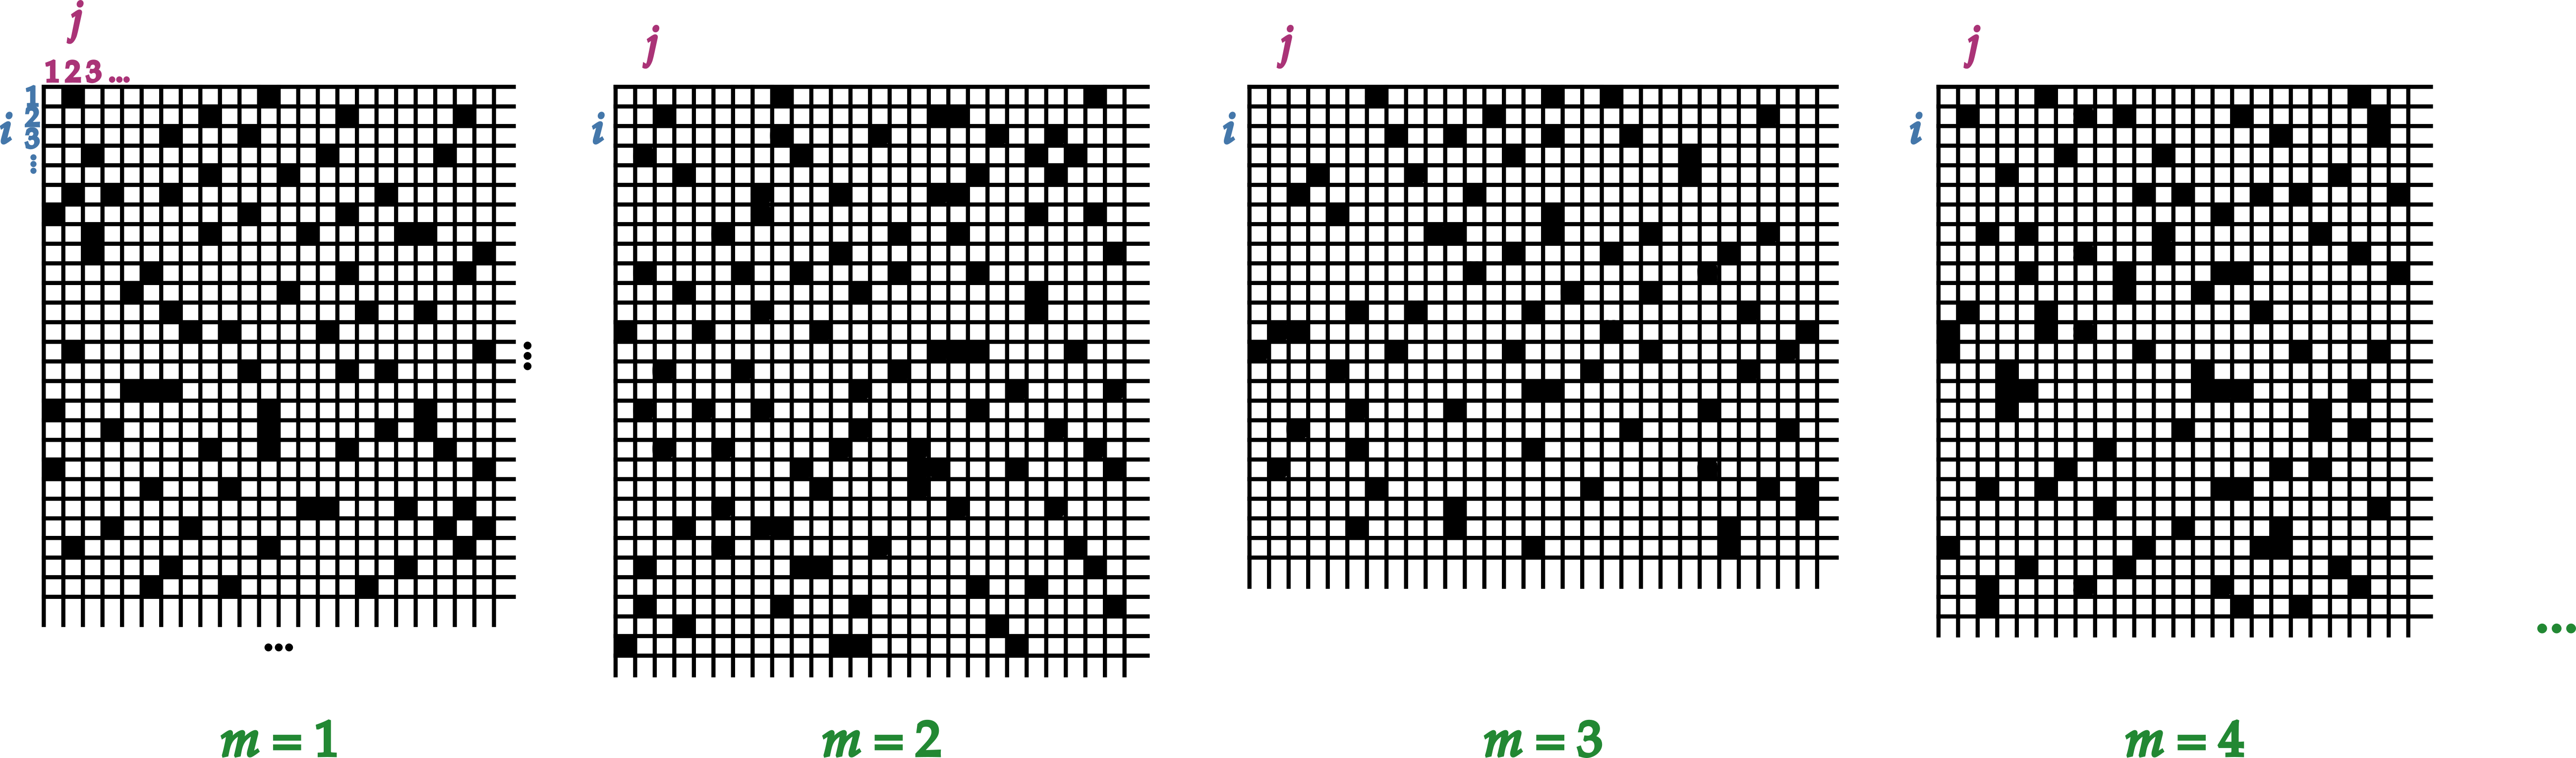
\includegraphics[width=\linewidth]{bente_notes_drawings.png}\\
 \caption{Imaginary layout of the connectivity from input to target region
   for all mice}\label{fig:cmij}
\end{figure}% bente_notes_drawings.svg

Mathematically we represent these statements and the grids of
\fig~\ref{fig:cmij} with the following quantities:
\begin{equation}
  \label{eq:quantity_connection}
  \yc_{ijm} =
  \begin{cases}
    1&\text{if neuron $i$ projects to neuron $j$ in mouse $m$},\\
    0&\text{if neuron $i$ doesn't project to neuron $j$ in mouse $m$}.
  \end{cases}
\end{equation}
Let's call them \emph{connections}.


For most of these statements we'll obviously never be able to ascertain
whether they're true or false. But they serve us well as basic statements:
we can precisely formulate our questions and data in terms of them.

\bigskip

The formulation just proposed is already based on some simplifications and
the neglect of possible hierarchies: we could have distinguished the
neurons in the two regions according to morphology or location, and the
mice according to age, weight, and so on. But I take it as a good starting
compromise between simplification and realism. We'll consider further
simplifications in the next step.

\subsection{Step 2: joint probability distribution for the connections}
\label{sec:step_joint_prob}


In order to assign the initial joint probability distribution
$\pf[(\yc_{ijm}) \| \yI]$, for all values of the connections $(\yc_{mij})$,
we explore the symmetries of our problem. Symmetries translate into
equalities of some values of the joint distribution, and therefore restrict
its possible values and mathematical form.

Let's give an example corresponding to the three-level
hierarchy~\ref{item:3-level} of \sect~\ref{sec:prelim_remarks}. If we
consider all input neurons $(i)$ to a specific target neuron $j$ in a
specific mouse $m$ as similar, then the joint probability should stay the
same under exchanges of the indices $i$ for which the connections have the
same values. For example:
\begin{multline}
  \label{eq:example_exchange_i}
  \pf(\yc_{2\,jm}=0, \yc_{5\,jm}=1, \yc_{6\,jm}=1, \yc_{9\,jm}=0 \| \yI) ={}\\
  \pf(\underbracket[0.5pt]{\yc_{9\,jm}=0, \yc_{5\,jm}=1, \yc_{6\,jm}=1, \yc_{2\,jm}=0}_{2\leftrightarrow 9} \| \yI) ={}\\
  \pf(\underbracket[0.5pt]{\yc_{2\,jm}=0, \yc_{6\,jm}=1, \yc_{5\,jm}=1, \yc_{9\,jm}=0}_{5\leftrightarrow 6} \| \yI) ={}\\
  \pf(\underbracket[0.5pt]{\yc_{9\,jm}=0, \yc_{6\,jm}=1, \yc_{5\,jm}=1, \yc_{2\,jm}=0}_{2\leftrightarrow 9,\quad 5\leftrightarrow 6} \| \yI).
\end{multline}
We can't exchange $i=2$ and $i=5$ because their connections have different
values. Because of this symmetry in $i$ the joint probability must have a
specific form, by de~Finetti's representation
theorem:\citep{definetti1930,hewittetal1955,heathetal1976,diaconis1977,diaconisetal1980,dawid2013}
\begin{equation}
  \label{eq:definetti_example_i}
  \pf[(\yc_{ijm}) \| \yI] =
  \int\!\!\!\prod_{jm}\Bigl[\di f_{jm}\;
  {f_{jm}}^{\sum_{i}\yc_{ijm}}\;(1-f_{jm})^{\sum_{i}(1-\yc_{ijm})}\Bigr]\;
  \pf[(f_{jm}) \| \yI].
\end{equation}
In this expression, $f_{jm}$ is the total number of neurons projecting to
target neuron $j$ in mouse $m$, and what remains to be assigned is the
probability distribution $\pf[(f_{jm}) \| \yI]$ over such numbers for all
$j$ and $m$. It may look like a complicated expression, but it has
considerably reduced the possible assignments of joint probabilities.

The second level of the hierarchy of this example was to consider a
similarity of connectivity statistics -- which are the quantities $f_{jo}$
-- among all target neurons in each specific mouse. This means that the
joint probability $\pf[(f_{jm}) \| \yI]$ in the formula above is symmetric
in the index $j$ for each fixed $m$. This leads, again by de~Finetti's
theorem, to a new expression similar to the one above, with new
$m$-dependent statistics as parameters and a joint distribution for htem.
The final level in the hierarchy says that this distribution is itself
symmetric in the index $m$, thus leading to a final integral expression in
terms of a single parameter only with an associated probability
distribution.

\bigskip

The difficulty of the three-level formulation just sketched is
mathematical: the integrals involved are over more complex spaces which are
numerically more expensive to handle.

As a first, simpler formulation we consider instead the more unrealistic
but powerful symmetry of example~\ref{item:1-level}: the joint distribution
$\pf[(\yc_{ijm}) \| \yI]$ stays the same under exchanges of \emph{any}
indices $(i,j,m)$ for which the connections have the same values. For example,
\begin{multline}
  \label{eq:example_exchange_i}
  \pf(\yc_{2\,3\,7}=0, \yc_{5\,5\,2}=1, \yc_{9\,1\,4}=0 \| \yI) =
  \pf(\yc_{9\,3\,7}=0, \yc_{5\,5\,2}=1, \yc_{2\,1\,4}=0 \| \yI) ={}\\
  \pf(\yc_{2\,1\,7}=0, \yc_{5\,5\,2}=1, \yc_{9\,3\,4}=0 \| \yI) =
  \pf(\yc_{2\,3\,4}=0, \yc_{5\,5\,2}=1, \yc_{9\,1\,7}=0 \| \yI) ={}\\
  \pf(\yc_{9\,1\,7}=0, \yc_{5\,5\,2}=1, \yc_{2\,3\,4}=0 \| \yI) =
  \dotsb\quad\text{and so on.}
\end{multline}
We can only exchange indices with the same connection values, but
we have full freedom otherwise.

Again by de~Finetti's theorem, this symmetry forces our joint probability
distribution to have this form:
\begin{equation}
  \label{eq:definetti_1level}
  \begin{split}
  \pf[(\yc_{ijm}) \| \yI] &=
  \int\!\!\!\di q\;
  q^{\sum_{i}\yc_{ijm}}\;(1-q)^{\sum_{i}(1-\yc_{ijm})}\;
  \pf(q \| \yI)
\\ &\equiv
  \int\!\!\!\di q\;
  q^{R f}\;(1-q)^{R\,(1-f)}\;
  \pf(q \| \yI)
\end{split}
\end{equation}




The symmetries briefly discussed previously

Let's analyse two approximate symmetries first. Consider a specific mouse
$m$.

For each neuron $i$ in the input region, we can approximately judge as
equally likely that it will connect to any of the neurons $j$ in the target
region. This means that our initial probability distribution should remain
the same if we swap some values of the index $j$, with $m$ and $i$ fixed.
For example, the probability that neuron \#\,3 in the input region projects
to neuron \#\,2 in the target region and does not project to neuron \#\,5
should be the same if we exchange 2 and 5 in that statement. And similarly
for combinations of such statements:
\begin{equation}
  \label{eq:example_exch_j}
  \pf(\yc_{m\,3\,2} \eq 1, \yc_{m\,3\,5} \eq 0 \| \yI )
=  \pf(\yc_{m\,3\,2} \eq 0, \yc_{m\,3\,5} \eq 1 \| \yI ).
\end{equation}
This symmetry is an approximation: if the indices $i$ and $j$ bear some
information about the neurons' locations, our probability should reflect
the possibility that nearby neurons may connect more easily, for example.

We have an analogous approximate symmetry under exchanges of the
input-neuron index $i$ for fixed target neuron $j$.

These two approximate symmetries together are important because they
greatly restrict the possible values of our initial probability
distribution $\pf[(\yc_{mij}) \| \yI]$. The result they lead
to\citep{hoover1979,aldous1981,diaconisetal1981b} is mathematically
difficult for me, however. To further simplify the problem I make an even
rougher approximation: that the symmetries above hold not just for $i$ and
$j$ separately, but for any pairs of them. This assumption is even more
unrealistic than the previous two, because it gives the same probability to
the situation where each input neuron is connected with only one, distinct,
target neuron, as to the situation where only one input neuron is connected
to all target neurons, and all other input neurons are unconnected.

With this approximation the joint probability distribution for a given
mouse $m$ assumes the following form, by de~Finetti's representation
theorem:\citep{definetti1930,hewittetal1955,heathetal1976,diaconis1977,diaconisetal1980,dawid2013}.
Take a set of $k_{m}$ input neurons and $l_{m}$ target neurons, and
consider all possible connections $\yc_{mij}$ between them, with
$i=1,\dotsc,k_{m}$ and $j=1,\dotsc,l_{m}$. Then
\begin{equation}
  \label{eq:definetti_ij}
  \begin{split}
  \pf[(\yc_{mij}) \| m, \yI] &=
  \int_{0}^{1}\!\!\!\!\di\nu_{m}\;\pf(\nu_{m} \| \yI)\;
  \prod_{ij}\bigl[
  {\nu_{m}}^{\yc_{mij}}\;(1-\nu_{m})^{1-\yc_{mij}}
  \bigr]
  \\
  &\equiv \int_{0}^{1}\!\!\!\!\di\nu_{m}\;\pf(\nu_{m} \| \yI)\;
  {\nu_{m}}^{k_{m}l_{m}\yf_{m}}\;
  (1-\nu_{m})^{k_{m}l_{m}(1-\yf_{m})}.
\end{split}
\end{equation}
Here $k_{m}l_{m}\yf_{m} = \sum_{ij} \yc_{mij}$ is the total number of
connections between the $k_{m}$ input neurons and the $l_{m}$ target
neurons, and $0\le \nu_{m} \le 1$ is the population-averaged number of
connections from the \emph{whole} input region to the \emph{whole} target
region. The probability distribution $\pf(\nu_{m} \| I)$ expresses our
beliefs about the total number of connections from input to target region
in mouse $m$. The formula above is valid only if $k_{m}$ and $l_{m}$ are
small (say, one tenth at most) compared to their region sizes.



\bigskip


Let's see how our question and data can be expressed in term of these
statements and the quantities $(\yc_{mij})$.

We imagine to check every neuron $i$ in the target region of every mouse
$m$. For each such neuron we count how many neurons from the input region
project to it. Let's call this number $\yN_{mi}$. From the point of view of
\fig~\ref{fig:cmij} we're considering every column from every grid, in
turn, and counting how many black entries it has. If we were able to
perform these observations, at the end we could build a histogram of the
numbers $(\yN_{mi})$, showing the proportion of neurons in the target
region that have $0$ inputs from the input region, or $1$ input, $2$
inputs, $n$ inputs, and so on. These values would be the bins of the
histogram. The number of bins is large -- as much as the largest number of
neurons that could make the input region of a mouse. Denote by $F_{n}$ the
proportion (between $0$ and $1$) of neurons that receive $n$ inputs. This
proportion is calculated from all numbers $(\yN_{mi})$ by
\begin{equation}
  \label{eq:histogram_from_N}
F_{n} =
\frac{\sum_{mi}\delt(\yN_{mi}=n)}{\sum_{m}L_{m}} \equiv
  \frac{\text{\small number of $\yN_{mi}$s equal to $n$}}
  {\text{\small total number of neurons in target regions}}.
\end{equation}
The whole histogram is the set of proportions
$\yF \defd (F_{0}, F_{1}, \dotsc)$.


This histogram can give one definite meaning to the question \enquote{how
  many inputs from the input region does a neuron in the target region have
  on average?}: we are asking \enquote{what the mean of the histogram?},
that is,
\begin{equation}
  \label{eq:mean_histogram}
  \text{\small average number of inputs} =
  \sum_{n}n\,F_{n} \equiv \frac{\sum_{mi}\yN_{mi}}{\sum_{m}L_{m}}.
\end{equation}
But the histogram would tell us even more, for example the percentage of
target neurons that receive between $100$ and $200$ inputs from the input
region, obtained by summing $F_{100} + \dotsb + F_{200}$.

It's good to keep in mind that our question could also be approached in
slightly different ways, leading to different secondary questions. For
example, we could construct a histogram for the number of inputs for each
mouse individually, thus obtaining several
$\yF^{(m)}=\bigl(F^{{m}}_{0}, F^{{m}}_{1}, \dotsc)$, one for each $m$. Then
we could ask: \enquote{what is the average connectivity histogram for a
  mouse?}, that is,
\begin{equation}
  \label{eq:average_histogram_per_mouse}
  \frac{1}{\text{\footnotesize number of mice}}\sum_{m}\; \yF^{(m)}
\end{equation}
and also ask how much such histogram can vary from mouse to mouse.

\medskip

These alternative questions are important in view of possible
approximations in our assumptions and maths.



For example, if we assume that
all target neurons from all mice can be somehow pooled together -- which
makes the maths easier -- then we are forsaking the possibility of
analysing the individual connectivity histograms.

\medskip

Although we'll never be able to construct such a histogram, we can
nevertheless guess, from our observations in a small set of mice, what kind
of shape and numerical values it could have. So our goal is to determine
the probability
\begin{equation}
  \label{eq:prob_histogram_general}
  \pf(\text{\small histogram} \| \text{\small data}, \yI)
\end{equation}
for each possible histogram, given the data collected in our observations
and any other information $\yI$ we have, including our present knowledge of
brain biology.

These probability above can be found using the rule for conditional
probabilities:
\begin{equation}
  \label{eq:prob_histogram_bayes}
  \pf(\text{\small histogram} \| \text{\small data}, \yI)
  \propto
  \pf(\text{\small data} \| \text{\small histogram}, \yI)
  \times
  \pf(\text{\small histogram} \|  \yI).
\end{equation}
To calculate these we need to determine our initial probability
distribution $\pf(\text{\small histogram} \| \yI)$ for all possible
histograms. In fact we need to determine the initial probability of a
couple more things, for example the total number of neurons in the input
region $K_{m}$, for each mouse $m$. All other probabilities are calculated
from this initial probability distribution.

In the next section we discuss and analyse several alternative assumptions
that we can use to build the distribution
$\pf(\text{\small histogram} \| \yI) \equiv \pf(\yF \| \yI)$. Some of these
assumptions are approximate or unrealistic, yet unfortunately necessary for
making the problem mathematically tractable. After discussing the
alternatives we'll choose specific ones to arrive at formulae that we can
use with the data. The discussion of the alternatives is useful because we
can step back and try to change the less realistic assumptions if we see
that our formulae don't work well.


\section{Initial probability distribution}
\label{sec:init_prob}

The assumptions we use to build our initial probability distribution
$\pf(\yF \| \yI)$ are about the symmetries of our problem.

The first symmetry is very intuitive and compelling. Take the distribution
of numbers of inputs for a given mouse $m$: $(\yN_{m1}, \yN_{m2})$ ***



In order to formulate the initial probability distribution $\pf[(\yc_{mij})
\| \yI]$ we explore the symmetries of our problem.

Let's analyse two approximate symmetries first. Consider a specific mouse
$m$.




\clearpage
\hrule




the answers to our
question~\ref{item:Q2} and the statement of our experimental observations
are built up from the specific statements~\eqref{eq:statement_connection}.
For example, the statement \statm{In mouse \#\,3, neuron \#\,1 in the
  target region receives input from 2 neurons in the input region} is
equivalent to the composite statement \statm{In mouse \#\,3, neuron \#\,1
  in the target region receives input from neurons \#\,1 and \#\,2, or
  \#\,1 and \#\,3, or \#\,1 and \#\,4, or \ldots\ in the input region},
which we can express as
\begin{multline}
  (\yC_{311} \mathbin{\text{and}} \yC_{312}) \mathbin{\text{or}}
  (\yC_{311} \mathbin{\text{and}} \yC_{313}) \mathbin{\text{or}}
  \dotsb{}\\ {}\mathbin{\text{or}}
  (\yC_{312} \mathbin{\text{and}} \yC_{313}) \mathbin{\text{or}}
  (\yC_{312} \mathbin{\text{and}} \yC_{314}) \mathbin{\text{or}}
  \dotsb{}
\end{multline}





 Let's denote such kind of statement with
\begin{equation}
  \label{eq:statement_connection}
  \yC_{mij} \defd \parbox[t]{0.8\linewidth}{\statm{In mouse $m$, neuron $i$ in input region projects to neuron $j$ in target region}}
\end{equation}
and let's introduce the quantity
\begin{equation}
  \label{eq:quantity_connection}
  \yc_{mij} =
  \begin{cases}
    1&\text{if $\yC_{mij}$ is true},\\
    0&\text{if $\yC_{mij}$ is false}.
  \end{cases}
\end{equation}











We can rephrase it in
two different ways; it's the second that probably interests us:

\begin{enumerate}[label=\textbf{Q\arabic*}.,ref=Q\arabic*]
  \item\label{item:Q1} If we examine a new neuron in region $A$ in a new
  mouse, how many neurons in region $B$ will project to it? The possible
  answers to this question are: $0$, $1$, $2$, and so on.
  \item\label{item:Q2} If we examine all neurons in region $A$ in a very
  large sample of mice, and for each neuron we count how many neurons from
  region $B$ project to it, then what are the frequencies with which we'll
  observe $0$ connections, $1$ connection, $2$ connections, and so on? One
  possible answer could be this distribution:
  \[\text{0: }0.1\%, \quad \text{1: }0.3\%, \quad\dotsc,
    \quad \text{1\,000: }24\%, \quad \dotsc\]
  another answer could be this distribution:
  \[\text{0: }0.02\%, \quad \text{1: }0.07\%, \quad\dotsc,
    \quad \text{1\,000: }31\%, \quad \dotsc\]
  and so on, for all possible distributions of frequencies.
\end{enumerate}
For the first question we must give a distribution of probability over all
possible answers $0$, $1$, and so on. For the second the probability is
distributed over all possible frequency distributions.

The answers to these two questions and their probabilities are connected;
in particular, from the second we can obtain the first. The second is more
informative, because it gives us also a range of variability.

Our analysis will also produce probabilities for other another quantity:
how many neurons are there in region $B$, in the next mouse we observe?


We must consider the set of mice that have been observed and those that will
be observed in the future. Let's label each mouse with an index $m$. For
our inferences to be valid, these mice must be judged \enquote{similar}.

Now that we've labelled the mice and their neurons in the two regions, we
can make several concrete statements, such as
\[\parbox{0.95\linewidth}{\statm{In mouse \#\,64, the neuron \#\,931 in the input
      region projects to the neuron \#\,1\,488 in the target region.}}\]
which can be either true or false. Let's denote such kind of statement with
\begin{equation}
  \label{eq:statement_connection}
  \yC_{mij} \defd \parbox[t]{0.8\linewidth}{\statm{In mouse $m$, neuron $i$ in input region projects to neuron $j$ in target region}}
\end{equation}
and let's introduce the quantity
\begin{equation}
  \label{eq:quantity_connection}
  \yc_{mij} =
  \begin{cases}
    1&\text{if $\yC_{mij}$ is true},\\
    0&\text{if $\yC_{mij}$ is false}.
  \end{cases}
\end{equation}


Obviously for most of these statements we'll never be able to ascertain
whether they're true or false. But the answers to our
question~\ref{item:Q2} and the statement of our experimental observations
are built up from the specific statements~\eqref{eq:statement_connection}.
For example, the statement \statm{In mouse \#\,3, neuron \#\,1 in the
  target region receives input from 2 neurons in the input region} is
equivalent to the composite statement \statm{In mouse \#\,3, neuron \#\,1
  in the target region receives input from neurons \#\,1 and \#\,2, or
  \#\,1 and \#\,3, or \#\,1 and \#\,4, or \ldots\ in the input region},
which we can express as
\begin{multline}
  (\yC_{311} \mathbin{\text{and}} \yC_{312}) \mathbin{\text{or}}
  (\yC_{311} \mathbin{\text{and}} \yC_{313}) \mathbin{\text{or}}
  \dotsb{}\\ {}\mathbin{\text{or}}
  (\yC_{312} \mathbin{\text{and}} \yC_{313}) \mathbin{\text{or}}
  (\yC_{312} \mathbin{\text{and}} \yC_{314}) \mathbin{\text{or}}
  \dotsb{}
\end{multline}

The probabilities of such combinations are completely determined once we
give an initial joint probability distribution for all
statements~\eqref{eq:statement_connection} and their negations, which is
equivalent to the joint distribution of 
\begin{equation}
  \pf[(\yc_{mij}) \| \yI] \equiv
  \pf(\yc_{111}, \yc_{112},\yc_{113},\dotsc \| \yI)
  \label{eq:main_init_prob}
\end{equation}
conditional on the information $\yI$ that we have before doing the
experiments and the observations.

Now, we'll want the probability of a specific answer $A$ to our question,
conditional on the data $D$ we observed: $\pf(A \| D,\yI)$. By the rule of
conditional probability we obtain it as
\begin{equation}
  \label{eq:Bayes_main}
  \pf(A \| D \mathbin{\text{and}} \yI) =
\frac{\pf(A \mathbin{\text{and}} D \| \yI)}{\pf(D \| \yI)}.
\end{equation}
The probabilities in the  numerator and denominator can be obtained from
our main joint probability~\eqref{eq:main_init_prob} using the basic rules
of the probability-calculus.

\medskip

So our strategy is as follows:
\begin{enumerate}
\item Quantitatively determine the initial joint probability
  $\pf[(\yc_{mij}) \| \yI]$.
\item Resolve the answers to question~\ref{item:Q2} in terms of the basic
  statements $\yC_{mij}$.
\item Resolve the experimental observations in terms of the basic
  statements $\yC_{mij}$.
\item Calculate the probabilities in~\eqref{eq:Bayes_main}.
\end{enumerate}

We now face these steps in turn. We shall discuss several possible
alternative assumptions and conceptual or mathematical approximations that
we can make in order to proceed.

\section{Initial probability distribution}
\label{sec:init_prob}

In order to formulate the initial probability distribution $\pf[(\yc_{mij})
\| \yI]$ we explore the symmetries of our problem.

Let's analyse two approximate symmetries first. Consider a specific mouse
$m$.

For each neuron $i$ in the input region, we can approximately judge as
equally likely that it will connect to any of the neurons $j$ in the target
region. This means that our initial probability distribution should remain
the same if we swap some values of the index $j$, with $m$ and $i$ fixed.
For example, the probability that neuron \#\,3 in the input region projects
to neuron \#\,2 in the target region and does not project to neuron \#\,5
should be the same if we exchange 2 and 5 in that statement. And similarly
for combinations of such statements:
\begin{equation}
  \label{eq:example_exch_j}
  \pf(\yc_{m\,3\,2} \eq 1, \yc_{m\,3\,5} \eq 0 \| \yI )
=  \pf(\yc_{m\,3\,2} \eq 0, \yc_{m\,3\,5} \eq 1 \| \yI ).
\end{equation}
This symmetry is an approximation: if the indices $i$ and $j$ bear some
information about the neurons' locations, our probability should reflect
the possibility that nearby neurons may connect more easily, for example.

We have an analogous approximate symmetry under exchanges of the
input-neuron index $i$ for fixed target neuron $j$.

These two approximate symmetries together are important because they
greatly restrict the possible values of our initial probability
distribution $\pf[(\yc_{mij}) \| \yI]$. The result they lead
to\citep{hoover1979,aldous1981,diaconisetal1981b} is mathematically
difficult for me, however. To further simplify the problem I make an even
rougher approximation: that the symmetries above hold not just for $i$ and
$j$ separately, but for any pairs of them. This assumption is even more
unrealistic than the previous two, because it gives the same probability to
the situation where each input neuron is connected with only one, distinct,
target neuron, as to the situation where only one input neuron is connected
to all target neurons, and all other input neurons are unconnected.

With this approximation the joint probability distribution for a given
mouse $m$ assumes the following form, by de~Finetti's representation
theorem:\citep{definetti1930,hewittetal1955,heathetal1976,diaconis1977,diaconisetal1980,dawid2013}.
Take a set of $k_{m}$ input neurons and $l_{m}$ target neurons, and
consider all possible connections $\yc_{mij}$ between them, with
$i=1,\dotsc,k_{m}$ and $j=1,\dotsc,l_{m}$. Then
\begin{equation}
  \label{eq:definetti_ij}
  \begin{split}
  \pf[(\yc_{mij}) \| m, \yI] &=
  \int_{0}^{1}\!\!\!\!\di\nu_{m}\;\pf(\nu_{m} \| \yI)\;
  \prod_{ij}\bigl[
  {\nu_{m}}^{\yc_{mij}}\;(1-\nu_{m})^{1-\yc_{mij}}
  \bigr]
  \\
  &\equiv \int_{0}^{1}\!\!\!\!\di\nu_{m}\;\pf(\nu_{m} \| \yI)\;
  {\nu_{m}}^{k_{m}l_{m}\yf_{m}}\;
  (1-\nu_{m})^{k_{m}l_{m}(1-\yf_{m})}.
\end{split}
\end{equation}
Here $k_{m}l_{m}\yf_{m} = \sum_{ij} \yc_{mij}$ is the total number of
connections between the $k_{m}$ input neurons and the $l_{m}$ target
neurons, and $0\le \nu_{m} \le 1$ is the population-averaged number of
connections from the \emph{whole} input region to the \emph{whole} target
region. The probability distribution $\pf(\nu_{m} \| I)$ expresses our
beliefs about the total number of connections from input to target region
in mouse $m$. The formula above is valid only if $k_{m}$ and $l_{m}$ are
small (say, one tenth at most) compared to their region sizes.

\medskip

The probability distribution for the connections present in different mice
can be obtained by combining the expressions above for each $m$. To do this
we need the initial joint probability distribution
\begin{equation}\label{eq:joint_nu_generic}
  \pf[(\nu_{m}) \| \yI]
  \equiv \pf(\nu_{1}, \nu_{2}, \dotsc \| \yI)
\end{equation}
for the total number of connections in several mice.

Our question has another symmetry, more realistic than the previous two. We
don't believe any of the mice to be examined to be special with respect to
the others, nor we do believe that the particular order in which they are
observed has any relevance. This means that our initial probability
distribution above should be invariant with respect to permutations of the
index $m$. Then we obtain the following expression, again by de~Finetti's
theorem:
\begin{equation}\label{eq:joint_nu_definetti}
  \pf[(\nu_{m}) \| \yI] =
  \int\!\!\!\di\yth\;\pf(\yth \| \yI)\;
  \prod_{m}  \yq(\nu_{m} \| \yth),
\end{equation}
where $\yq$ is a distribution that depends on the parameter $\yth$, and
$\pf(\yth \| \yI)$ is our initial probability distribution for this
parameter.

The parameter $\yth$ in principle represents every possible distribution --
or histogram -- of the total number of connections across the mice. For
example, a particular $\yth$ can say that 7\% of mice had $10^6$
connections, 11\% had $5\times 10^{7}$ connections, and so on. The above
formula sums over all such possible distributions. There is an infinite of
such distributions, so the integral is over an infinite-dimensional space.
When we calculate this integral with this full generality, we're using a
so-called \emph{non-parametric} method. But for mathematical simplicity we
can also decide to restrict our attention to histograms of specific shape,
such as a normal for example. In this case the integral is restricted to a
finite-dimensional space and we're using a \emph{parametric} method.

\medskip

Combining the initial probability distributions~\eqref{eq:definetti_ij} and
\eqref{eq:joint_nu_definetti} we finally obtain our initial probability
distribution for a joint set of statements $(\yC_{mij})$:
\begin{equation}
  \label{eq:main_init_prob_simplified}
    \pf[(\yc_{mij}) \| \yI] =
    \iint\!\!\!\di\yth\;\di\ynu\;
    \pf(\yth \| \yI)\;
    \prod_{mij}\Bigl[ \yq(\nu_{m} \| \yth)\;
  {\nu_{m}}^{\yc_{mij}}\;(1-\nu_{m})^{1-\yc_{mij}}
  \Bigr],
\end{equation}
where $\ynu \defd (\nu_{m})$.



\section{Statements of the questions and of the data}
\label{sec:statements_question_data}














\textcolor{white}{If you find this you can claim a postcard from me.}



%%%% examples use empheq
%   \begin{empheq}[left={\mathllap{\begin{aligned}    \de\yF_{\yc}/\de\yp&=0\text{:} \\
%         \de\yF_{\yc}/\de\ym&=0\text{:}\\ \de\yF_{\yc}/\de\yl&=0\text{:}\end{aligned}}\qquad}\empheqlbrace]{align}
%     \label{eq:con_p}
% %    \de\yF_{\yc}/\de\yp &\equiv
%     -\ln\yp + \ln\yq + \yl\yM + \ym\yu &=0,\\
%     \label{eq:con_u}
% %    \de\yF_{\yc}/\de\ym &\equiv
%     \yu\yp-1 &=0,\\
%     \label{eq:con_l}
%     %\de\yF_{\yc}/\de\yl &\equiv
%     \yM\yp-\yc &=0.
%   \end{empheq}
%%%%
% \begin{empheq}[box=\widefbox]{equation}
%   \label{eq:maxent_question}
%   \p\bigl[\yE{N+1}{k} \bigcond \tsum\yo\yf{N}\in\yA, \yM\bigr] = \mathord{?}
% \end{empheq}



% \[
%   \begin{tikzcd}
%       M_{n,n}(\CC) \arrow{r}{R'_{a}(\Hat{U})} & M_{n,n}(\CC)
%     \\
%     L(\mathcal{H}) \arrow{r}{\Hat{U}} \arrow[swap]{d}{R_*}\arrow[swap]{u}{R'_*} & L(\mathcal{H}) \arrow{d}{R_*}\arrow{u}{R'_*} \\
%       M_{n,n}(\CC) \arrow{r}{R_{a}(\Hat{U})} & M_{n,n}(\CC)
%   \end{tikzcd}
% \]

% \[
%   \begin{tikzcd}
%       \CC^n \arrow{r}{R'_*(A)} & \CC^n
%     \\
%     \mathcal{H} \arrow{r}{A} \arrow[swap]{d}{R}\arrow[swap]{u}{R'} & \mathcal{H} \arrow{d}{R}\arrow{u}{R'} \\
%       \CC^n \arrow{r}{R_*(A)} & \CC^n
%   \end{tikzcd}
% \]


% \[
%   \begin{tikzcd}
%     \mathcal{H} \arrow{r}{A} \arrow[swap]{d}{R} & \mathcal{H} \arrow{d}{R} \\
%       \CC^n \arrow{r}{R_*(A)} & \CC^n
%   \end{tikzcd}
% \]

%%\setlength{\intextsep}{0.5ex}% with wrapfigure
%\begin{figure}[p!]%{r}{0.4\linewidth} % with wrapfigure
%  \centering\includegraphics[trim={12ex 0 18ex 0},clip,width=\linewidth]{maxent_saddle.png}\\
%\caption{caption}\label{fig:comparison_a5}
%\end{figure}% exp_family_maxent.nb


%%%%%%%%%%%%%%%%%%%%%%%%%%%%%%%%%%%%%%%%%%%%%%%%%%%%%%%%%%%%%%%%%%%%%%%%%%%%
%%% Acknowledgements
%%%%%%%%%%%%%%%%%%%%%%%%%%%%%%%%%%%%%%%%%%%%%%%%%%%%%%%%%%%%%%%%%%%%%%%%%%%% 
\iffalse
\begin{acknowledgements}
  \ldots to Mari \amp\ Miri for continuous encouragement and affection, and
  to Buster Keaton and Saitama for filling life with awe and inspiration.
  To the developers and maintainers of \LaTeX, Emacs, AUC\TeX, Open Science
  Framework, R, Python, Inkscape, Sci-Hub for making a free and impartial
  scientific exchange possible.
%\rotatebox{15}{P}\rotatebox{5}{I}\rotatebox{-10}{P}\rotatebox{10}{\reflectbox{P}}\rotatebox{-5}{O}.
%\sourceatright{\autanet}
\mbox{}\hfill\autanet
\end{acknowledgements}
\fi

%%%%%%%%%%%%%%%%%%%%%%%%%%%%%%%%%%%%%%%%%%%%%%%%%%%%%%%%%%%%%%%%%%%%%%%%%%%%
%%% Appendices
%%%%%%%%%%%%%%%%%%%%%%%%%%%%%%%%%%%%%%%%%%%%%%%%%%%%%%%%%%%%%%%%%%%%%%%%%%%% 
\clearpage
% %\renewcommand*{\appendixpagename}{Appendix}
% %\renewcommand*{\appendixname}{Appendix}
% %\appendixpage
% \appendix

%%%%%%%%%%%%%%%%%%%%%%%%%%%%%%%%%%%%%%%%%%%%%%%%%%%%%%%%%%%%%%%%%%%%%%%%%%%%
%%% Bibliography
%%%%%%%%%%%%%%%%%%%%%%%%%%%%%%%%%%%%%%%%%%%%%%%%%%%%%%%%%%%%%%%%%%%%%%%%%%%% 
\defbibnote{prenote}{{\footnotesize (\enquote{de $X$} is listed under D,
    \enquote{van $X$} under V, and so on, regardless of national
    conventions.)\par}}
% \defbibnote{postnote}{\par\medskip\noindent{\footnotesize% Note:
%     \arxivp \mparcp \philscip \biorxivp}}

\printbibliography[prenote=prenote%,postnote=postnote
]

\end{document}

%%%%%%%%%%%%%%%%%%%%%%%%%%%%%%%%%%%%%%%%%%%%%%%%%%%%%%%%%%%%%%%%%%%%%%%%%%%%
%%% Cut text (won't be compiled)
%%%%%%%%%%%%%%%%%%%%%%%%%%%%%%%%%%%%%%%%%%%%%%%%%%%%%%%%%%%%%%%%%%%%%%%%%%%% 


%%% Local Variables: 
%%% mode: LaTeX
%%% TeX-PDF-mode: t
%%% TeX-master: t
%%% End: 
